\documentclass{article}

\usepackage{tikz}
\usetikzlibrary{spy,arrows}

\usepackage[font={small,sf},labelfont={bf},labelsep=endash]{caption}
\usepackage{sansmath}
\DeclareCaptionFormat{thesis}{\sansmath #1#2#3}
\captionsetup{format=thesis}

\usepackage{siunitx}

\begin{document}

\begin{sansmath}
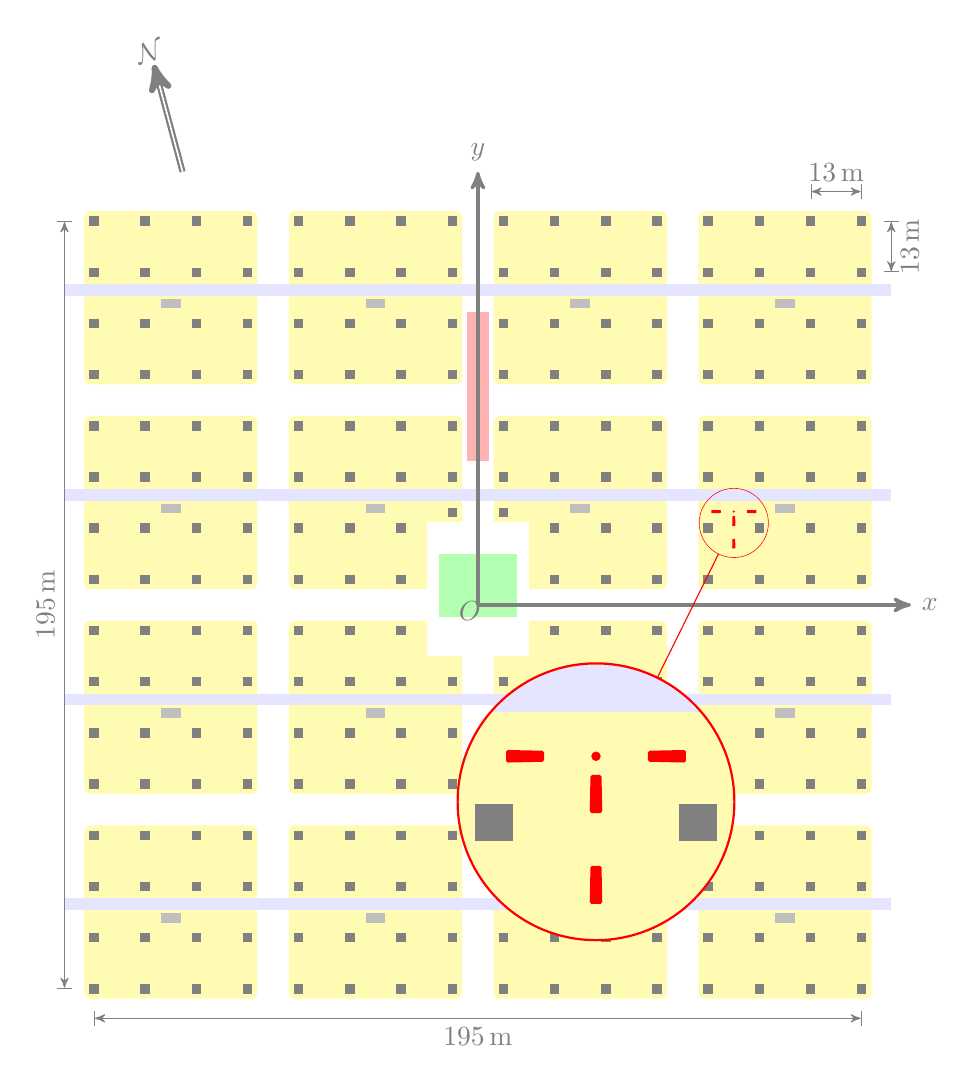
\begin{tikzpicture}
    [ x=.5mm, y=.5mm,
      font={\sffamily},
      station/.style={fill=gray},
      hut/.style={fill=lightgray},
      cluster/.style={fill=yellow!30, rounded corners=2pt},
      road/.style={fill=blue!10},
      calorimeter/.style={fill=green!30},
      tracker/.style={fill=red!30},
      hisparc/.style={fill=red, rounded corners=.15pt},
      hisparcgps/.style={fill=red},
      axis/.style={gray,very thick,->,>=stealth'},
      ruler/.style={gray,|<->|,>=stealth'},
      spy using outlines={red, circle, magnification=4, size=25 * 4, connect spies}
    ]
    \def\hisparcbox{%
        \path[hisparc]
            (-.4, .7) .. controls (0, .75) ..  (.4, .7) --
            (.35, -1.7) ..  controls(0, -1.72) ..  (-.35, -1.7) -- cycle;
    }

    % Clusters
    \foreach \i in {-1.5, -0.5, ..., 1.5} {
        \foreach \j in {-1.5, -0.5, ..., 1.5} {
            \path[cluster, shift={(\i * 52, \j * 52)}]
                (-22, -22) rectangle (22, 22);
        }
    }

    % Roads
    \foreach \i in {-1.5, -0.5, ..., 1.5} {
        \path[road, shift={(0, \i * 52 + 2)}]
            (-105, -1.5) rectangle (105, 1.5);
    }

    % Detector array
    \foreach \i in {-7.5, -6.5, ..., 7.5} {
        \foreach \j in {-7.5, -6.5, ..., 7.5} {
            \path[station, shift={(\i * 13, \j * 13)}]
                (-1.2, -1.2) rectangle (1.2, 1.2);
        }
    }
    \path[station, shift={(-6.5, 23.5)}] (-1.2, -1.2) rectangle (1.2, 1.2);
    \path[station, shift={(6.5, 23.5)}] (-1.2, -1.2) rectangle (1.2, 1.2);

    % Electronic huts
    \foreach \i in {-1.5, -0.5, ..., 1.5} {
        \foreach \j in {-1.5, -0.5, ..., 1.5} {
            \path[hut, shift={(\i * 52, \j * 52 - 1.5)}]
                (-2.5, -1.2) rectangle (2.5, 1.2);
        }
    }

    % Central detector
    \fill[white] (-13, -13) rectangle (13, 21);
    \path[calorimeter, shift={(0, 5)}] (-10, -8) rectangle (10, 8);

    % Muon tracker
    \path[tracker, shift={(0, 4)}] (-2.7, 32.5) rectangle (2.7, 70.5);

    % HiSPARC station
    \begin{scope}[shift={(65.0, 15.05)}, rotate=180]
        \hisparcbox
    \end{scope}
    \begin{scope}[hisparc, shift={(65.0, 20.82)}, rotate=180]
        \hisparcbox
    \end{scope}
    \begin{scope}[hisparc, shift={(70.0, 23.71)}, rotate=-90]
        \hisparcbox
    \end{scope}
    \begin{scope}[hisparc, shift={(60.0, 23.71)}, rotate=90]
        \hisparcbox
    \end{scope}
    \path[hisparcgps, shift={(65.0, 23.71)}] (0, 0) circle (.3);

    \draw[axis] (0, 0) -- (110, 0) node[right] {$x$};
    \draw[axis] (0, 0) -- (0, 110) node[above] {$y$};
    \node[axis,below left=-5pt] at (0, 0) {$O$};
    \draw[ruler] (-97.5, -105) -- (97.5, -105) node[midway,below] {\SI{195}{\meter}};
    \draw[ruler] (84.5, 105) -- (97.5, 105) node[midway,above] {\SI{13}{\meter}};
    \draw[ruler] (-105, -97.5) -- (-105, 97.5) node[midway,above,sloped] {\SI{195}{\meter}};
    \draw[ruler] (105, 84.5) -- (105, 97.5) node[midway,below,sloped] {\SI{13}{\meter}};

    \def\r{40pt}
    \newcommand{\calck}[1]{\pgfmathsetmacro{\k}{-#1 - 75 - 180}}
    \begin{scope}[gray,shift={(-75,110)}]
        \calck{0}
        \draw[thick,double,->,>=stealth'] (0,0) -- (\k:\r);
        \path (0,0) -- (\k:\r + 5pt) node[pos=1,rotate=-90,allow upside down,sloped] {$\mathcal{N}$};
    \end{scope}

    % Spy
    \spy on (65.0, 20.82) in node at (30, -50);

\end{tikzpicture}
\end{sansmath}

\end{document}
